\documentclass{article}
\usepackage{blindtext}
\usepackage{graphicx}

\title{Team 2 Proposal}
\date{2021 \\ February}

\author{Gabriel L., Jose Lazcano, Jesus Jaime, Yadiel, Fernando, Cristian}

\begin{document}

\maketitle
\section{Name, Place and Date}
ZeitNehmer Workflow Manager\\
Mayaguez, PR\\
Febrero 10, 2021
\section{Current Situation, Needs, Ideas and Concept}
\vspace{10}
Managers need project management programs to manage their employees tasks and projects and give them a way for them to know what they need to do. Most of these programs have become bloated over time and have overcomplicated tasks that should be pretty straightforward causing the need for managers to take training to be able to use these tools. The project would involved in creating a project management program that cuts the bloat and focuses on making an intuitive and easy to use platform where no training is needed to properly use. This would involve a structure where:
\begin{enumerate}
\item Platform for managers: Managers can access a platform to view tasks and projects and delegate them to employees.
\item Platform for employees: Employees can view tasks assigned to them and add notes alerting the manager of questions and or detailed info about the task.
\end{enumerate}
\section{Scope, Span and Synopsis}
\vspace{10}
The problem is to understand project management in general: deadlines, task lists, schedules, file sharing, communication, teamwork, and logistics of project management. This is used to build a theory of management systems: leadership, planning, project monitoring, status, standards and, improvement.

The project is to develop and research a Program Management Software. This project is expected to cover:
\begin{enumerate}
    \item project monitoring: team performance, task duration
    \item team collaboration
    \item task management: prioritize, strategic planning,  scheduling
    \item reporting
\end{enumerate}

\section{Assumptions and Dependencies}
\vspace{10}
Rough sketch requirements as user stories:
\begin{quotation}
    As a user, having an organized and productive workflow is very critical and important, because it drastically improves the productivity of the user and the company. When its time to divide the work withing a team or assigning work to your employees having a Workflow management app really helps the process. If someone is stuck in a task, they can show it on the app, so a manager/Leader can send him a message and start helping them. The employee/manager and the team-member/Leader communication improves by having the online message system.
\end{quotation}
\begin{quotation}
    As a user, having an easy-to-use and accessible Workflow Management app can be really helpful. I would like to be able to create and edit workflows as easy as possible, and to be remained about deadlines, messages and updates.
\end{quotation}

\section{Implicit/Derivative Goals}
\vspace{10}

Domain Requirements:
\begin{itemize}
    \item The data base must store end-user accounts, along with their password and personal information needed to create an account.
    \item The end-user should be able to create, edit, and delete current or new workflows.
    \item The end-user should be able to edit, update or delete their personal information from the data-base.
    \item The app should hide the personal information given by creating an account unless the end-user require it.
    \item The system-to-be needs to keep a list of every user registered so it can quickly identify if the user haves an account or it needs to create one.
    \item System-to-be must identify the user \“rank\” in order to classify the account as the manager or employee, as a leader or as a teammate.
    \item System-to-be must detect if end-user is active in on the page, for an online symbol that identify to other people that you are currently on the app and they can message you.
    \item System-to-be must detect & update the status of the task every time a user makes an update on their workflow.
    \item System-to-be must send push notification to the users notifying the deadlines, updates and messages.
\end{itemize}
\vspace{30}
Interface Requirements:

\begin{itemize}
    \item The system-to-be has a downtime of 15 minutes every 24 hours for a backup to save any changes of the website from the users, and storing important information on the data base.
    \item The system-to-be must store every workflow created in the data-base and update the ones that where changed.
    \item The system-to-be must show the workflows that are already stored, so end-users can identify and select witch one they want to work on.
    \item For security of the end-user account, the password should be initially obscured. They should have an option that enables the password to show for reviewing purposes.
\end{itemize}
For the system to work properly and ensure a good experience with the users it must comply with the following:
\begin{enumerate}
  \item Changes made will be updated at real time or with no more than a 200 ms delay for 99\% of the cases.
  \item Users will be notified about changes relating to their tasks as soon as it is updated.
  \item Even at peak times server load should be lower than 80\%
  \item Response times from interface must be kept lower than 500 ms.
  \item Platform must be available at all times, with the exclusion of programmed downtimes.
\end{enumerate}

\vspace{70}
Software Structure:

\begin{itemize}
    \item Security:

\vspace{5}
The Software will have the implementation of account registration, Users will provide an email and set up their accounts,
setting their password as Username. Once the account has been created and the User has logged in, User must select the
kind of work they will be focusing on and manage from available options. This includes:
\begin{enumerate}
    \item Sales
    \item Creative
    \item Marketing
    \item IT
    \item Finance
    \item Customer Service
    \item Software Development
    \item ECT
    \item Manufacturing
\end{enumerate}
Once
User has chosen their work, a link will be generated to invite other users to join on the workflow, input information
regarding the workflow.\\
\end{itemize}

\begin{itemize}
    \item Data Management:

    \vspace{5}
    Users also can Customize their main UI Workstation and save their settings
    Users can add widgets and tools to their
    work station
    The System tracks current events and their current status, from Ongoing to Complete.
    The System tracks Current Users that are online and their current workflows.
    System Monitors and sends notifications accordingly to constantly update the status of workflow.
\end{itemize}

\begin{itemize}
    \item Report Generation

    \vspace{5}
    TheSystem will track and report on the different workflows.
    This data is sent to the different users to their corresponding workflows.
    Users can
    update their workflows and report on their current state of their events.
    Messages can be sent to other users.
\end{itemize}
\vspace{5}
Domain Entities:
\begin{quotation}
    The entities methods take care of the invariants and rules of the entity instead of having those rules spread across the application layer.
    Every class has in own attributes and methods that will be called when the application is running but keeps it in an organized matter.
\end{quotation}
\bigbreak
\begin{figure}[ht!]
    \centering
    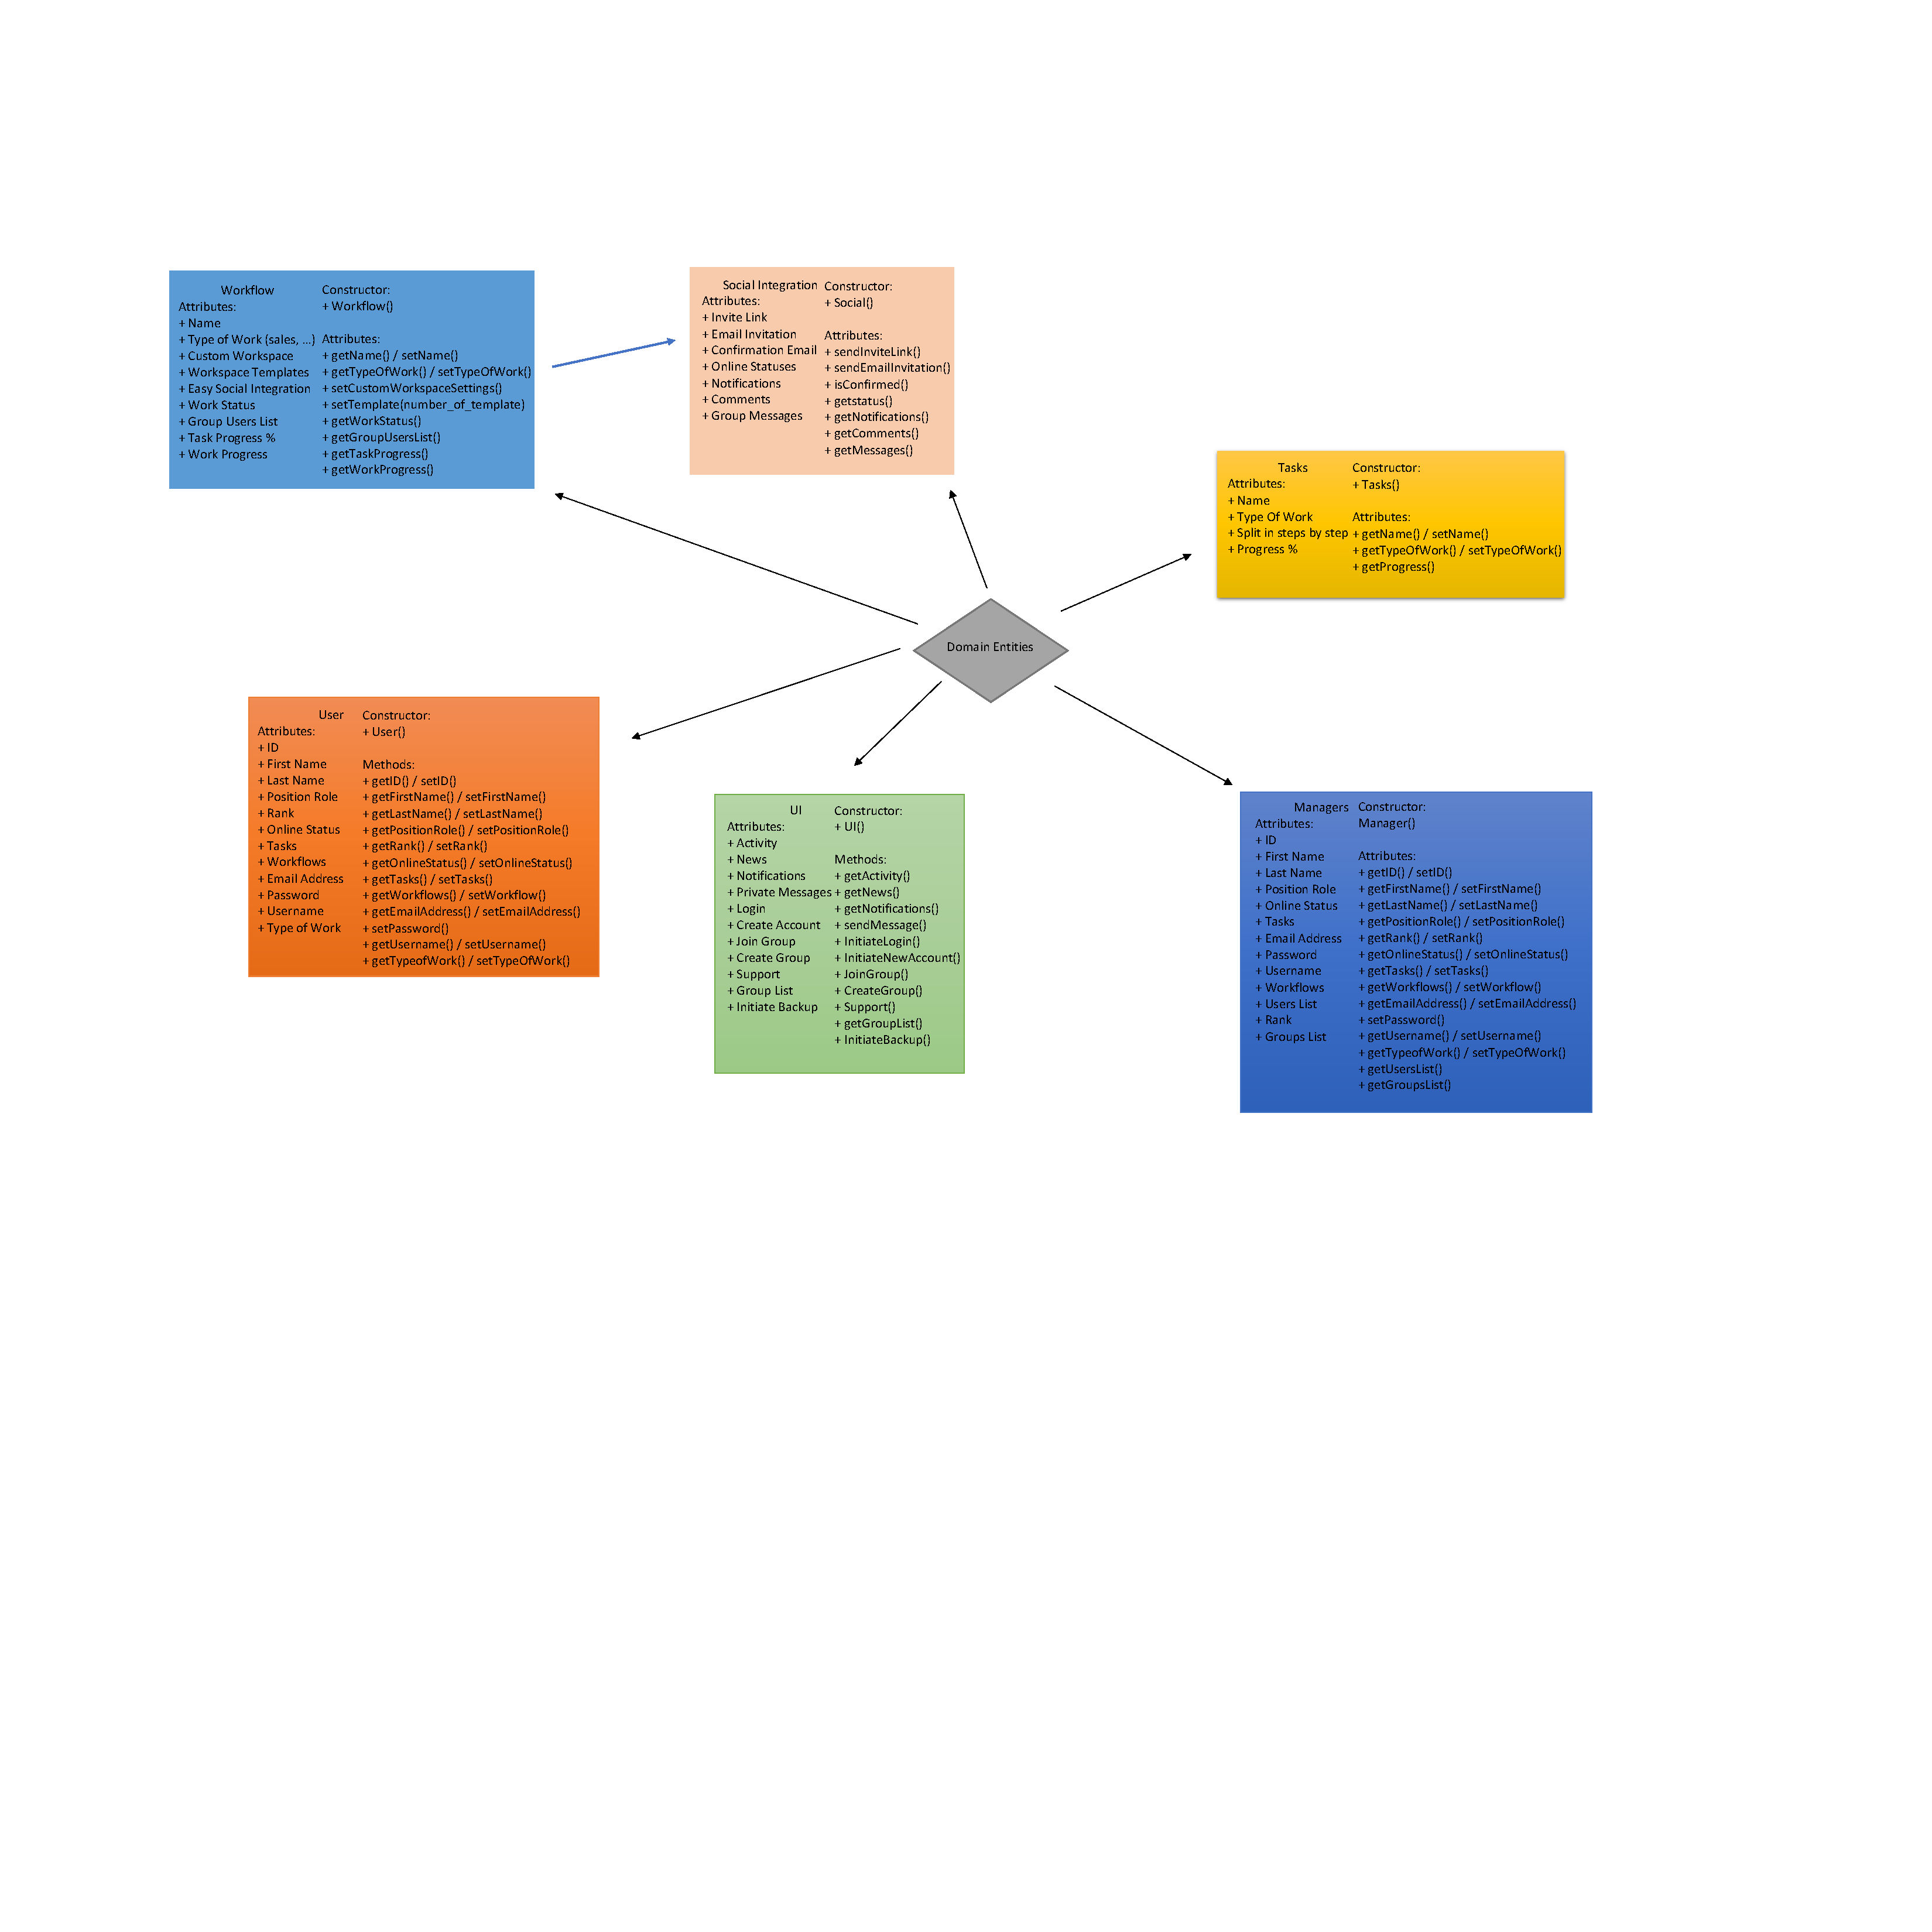
\includegraphics[width=1.2\columnwidth]{Images/Domain_Entities.pdf}
    \caption{Domain Entities}
    \label{fig:figure}
\end{figure}
\bigbreak
Domain Functions:
\begin{quotation}
    The domain functions takes care of the data when classes or variables get called when the user interacts with the platform.
    We can see this in the diagram below where we can view the navigation of the data between entities.
\end{quotation}
\bigbreak
\begin{figure}[ht!]
    \centering
    \includegraphics[width=0.5\columnwidth]{Images/state-view.pdf}
    \caption{Domain Entities}
    \label{fig:figure2}
\end{figure}
\bigbreak
\noindent Software Component Design:
\bigbreak
\noindent \textbf{module workflows:}
\begin{quote}
  \textbf{Variables:}
  \begin{quote}
    workflowName \textbf{String}; workflowDescription \textbf{String}; members \textbf{List}
  \end{quote}
  \textbf{Functions:}
  \begin{quote}

    status: boolean, status()
    \begin{quote}
      updates workflow current status, returns "ongoing" or "completed"
    \end{quote}

    currentlyOnline: List, currentlyOnline()
    \begin{quote}
      returns all users who are assigned to this task and are online.
    \end{quote}

    updateDescription: null, updateDescription(workflowDescriptions)
    \begin{quote}
     changes the workflow description.
    \end{quote}
  \end{quote}
\end{quote}
\textbf{end module}
\bigbreak

\noindent \textbf{module workflowManagement:}
\begin{quote}
  \textbf{Variables:}
  \begin{quote}
    username \textbf{String}; isManager \textbf{boolean}
  \end{quote}

  \textbf{Functions:}
  \begin{quote}

    createWorkflow: null, createWorkflow(isManager)
    \begin{quote}
      a new workflow is created, user must be a manager to do so.
    \end{quote}

    viewWorkflow: List, viewWorkflow(username, isManager)
    \begin{quote}
      views all workflows a certain user is currently on, must be a manager.
    \end{quote}

    onlineMembers: List, onlineMembers()
    \begin{quote}
      returns all members who are currently active.
    \end{quote}

  \end{quote}
\end{quote}
\textbf{end module}
\bigbreak

\noindent \textbf{module notifications:}
\begin{quote}
  \textbf{Variables:}
  \begin{quote}
    workflowName \textbf{String}; workflowMembers \textbf{List}
  \end{quote}

  \textbf{Functions:}
  \begin{quote}

    workflowUpdated: null, workFlowUpdated(workflowMembers, workflowName)
    \begin{quote}
      notifies all workflow memebers a change hasbeen made or status has changed.
    \end{quote}

    newWorkflow: null newWorkflow(workflowMembers)
    \begin{quote}
      notifies all members of the workflow that it has been created.
    \end{quote}

  \end{quote}
\end{quote}
\textbf{end module}
\bigbreak

\noindent \textbf{module accounts:}
\begin{quote}

  \textbf{Variables:}
  \begin{quote}
    email \textbf{String}; username \textbf{String}; department \textbf{String}; isManager \textbf{boolean}
  \end{quote}
  \textbf{Functions:}
  \begin{quote}

    changeDepartment: null, changeDepartment(department)
    \begin{quote}
      Switchs the user current department.
    \end{quote}


    managerStatus: boolean, managerStatus(isManager)
    \begin{quote}
      Assigns the user as a manager or as a regular user, returns manager status.
    \end{quote}

  \end{quote}
\end{quote}
\textbf{end module}

\section{Terminology}
\begin{center}

    \begin{tabular}{| l | p{5cm} |}\hline
    Term & Short definition \\ \hline
    Event & This can be referred as a task or job that the User has access to. \\ \hline
    User & Subject that enters and interacts with the system. \\ \hline
    System & This specifically refers to the software itself. \\ \hline
    UI & User Interface; Everything that the Users can see on display on the system. \\ \hline
    Workstation & The Workstation is the main User Interface where one will manage, access and configure the Users Workflow. \\ \hline
    Workflow & Page where all the social, working and management takes place. Each group provides workflows for each individual type ( sales
    , T I, ...). \\ \hline
    Social Integration & Provides social interaction between group members and users across the platform. Making the work environment very interactive
    and easier to use. \\ \hline
    Rank & A category assigned to the User. (i.e Manager, Student, Profesor, Employee). \\ \hline
    Downtime & A period of time when the platform is not available. \\ \hline
    \end{tabular}

\end{center}
\section{Roles}
\vspace{10}
\begin{center}

\begin{tabular}{| l | p{5cm} |}\hline
Name & Main Role \\ \hline
Gabriel L. & fetching information from the data-base\\ \hline
Yadiel     & Back-End\\ \hline
Cristian   & Front-end-design \\ \hline
Fernando   & Back-End \\ \hline
Jesus	   & Information storage\\ \hline
Jose Lazcano  & User Interface \\ \hline
\end{tabular}

\end{center}
\end{document}
